% ----------------------------------------------------------
% Vegood
% ----------------------------------------------------------
\chapter{Vegood} \label{cha:vegood}
Neste capítulo, apresentamos a aplicação Vegood, objeto deste trabalho. É sistema de arquitetura simples para dispositivos móveis, desenvolvido por meio de uma plataforma hibrida de forma a poder ser usado nas plataformas IOS 7+ e Android 4.2+, além  de integrada ao Facebook.

\section{Definição do produto} \label{sec:vegood:definicao}

O Vegood apresenta aos usuários uma rede social cuja temática é a culinária vegetariana e vegana, onde os usuários poderão publicar e disponibilizar receitas , além de  curtir , favoritar e comentar em receitas publicadas.

A aplicação possui duas formas de autenticação: uma através do próprio cadastro que poderá ser realizado no aplicativo, onde haverá uma tela de cadastro de usuário que preenche um formulário com os dados necessários para que uma conta seja criada; e uma outra, através do Facebook,  quando o usuário autoriza que a aplicação utilize as suas credenciais desta rede social para se logar. Após a autenticação o aplicativo abrirá sua tela principal.

O usuário também pode seguir e ser seguido por todos os usuários, assim criando um vínculo social dentro da aplicação. Além das funcionalidades já citadas, o Vegood também irá disponibilizar informações, dicas e mitos sobre o vegetarianismo. 

É importante ressaltar que a utilização plena da aplicação exige a conexão com a Internet.

\section{Modelagem do Sistema}
Nesta seção, apresentamos as etapas do desenvolvimento do Vegood, subdividido em: definição de funcionalidades, definição do escopo, coleta e análise de requisitos, modelagem e confecção de casos de uso e regras de negócios.

\subsection{Funcionalidades} \label{sec:vegood:Funcionalidades}
As funcionalidades correspondem às possíveis ações que o usuário poderá fazer no aplicativo. Na tabela a seguir estão as funcionalidades mais importantes do aplicativo:

\begin{table}[H]
	\centering
	\caption{Funcionalidades do Vegood}
	\label{funcionalidades-do-vegood}
	\begin{tabular}{|c|l|l|}
	\hline
	\textbf{Código} & \textbf{Funcionalidades} & \textbf{Descrição} \\ \hline
	F1  & \begin{tabular}[c]{@{}l@{}} Publicar Receita\end{tabular} & \begin{tabular}[c]{@{}l@{}} Criar um post contendo a receita, informando \\ o título, imagem, categoria, tempo de preparo \\ e cozimento, dificuldade, porções, ingredientes \\ necessários e modo de preparo.\end{tabular} \\ \hline
	F2  & \begin{tabular}[c]{@{}l@{}} Socializar com as publicações\end{tabular} & \begin{tabular}[c]{@{}l@{}} Interagir com as publicações do aplicativo, \\ possibilitando aos usuários curtir, \\ comentar e favoritar as receitas.\end{tabular} \\ \hline
	\end{tabular}
\end{table}


\subsection{Escopo} \label{sec:vegood:Escopo}
A aplicativo será gratuito e tem como finalidade principal o compartilhamento de receitas culinárias vegetarianas e veganas com seus usuários, aumentando as  opções de receitas para que estes façam a sua própria comida.

\subsection{Levantamento de requisitos} \label{sec:vegood:Levantamento de requisitos}

Segundo \citeauthor{pfleeger2004engenharia}, um requisito é uma característica do sistema ou a descrição de algo que o sistema é capaz de realizar para atingir os seus objetivos. Os requisitos podem ser classificados em varias formas. Tradicionalmente, os requisitos de software são classificados em Requisitos Funcionais (funcionalidades da aplicação) e Requisitos Não-Funcionais (características das funcionalidades).

\subsubsection{Requisitos funcionais} \label{sec:vegood: Requisitos funcionais}
Os requisitos funcionais são aqueles que fazem parte da aplicação, como um relatório específico ou um campo a mais em um cadastro. Eles normalmente têm a finalidade de atender uma demanda do usuário, possibilitando ou facilitando o seu trabalho. Requisitos funcionais são implementados na própria aplicação, sendo que o seu corpo é, em última análise, é o produto da conjunção destes requisitos.

\begin{table}[H]
	\centering
	\caption{Requisitos funcionais}
	\label{requisitos-funcionais}
	\begin{tabular}{|c|l|l|c|c|}
	\hline
	\textbf{Código} & \textbf{Requisitos} & \textbf{Descrição} & \textbf{Dependência} & \textbf{Impotância} \\ \hline
	 
		RF1 & Login & \begin{tabular}[c]{@{}l@{}} Permitir que o usuário \\ faça login pelo próprio \\ aplicativo  ou com suas \\ credenciais do Facebook.\end{tabular} & [RNF3] & Essencial \\ \hline
		 
		RF2 & Perfil & \begin{tabular}[c]{@{}l@{}} Permitir ao usuário visualizar \\ seu  perfil, quem seguir e \\ visualizar perfis de outros \\ usuários.\end{tabular} & [RNF3][RF1]		& Essencial \\ \hline
	 
		RF3 & Publicar receitas & \begin{tabular}[c]{@{}l@{}} Permitir ao usuário criar \\ receitas e publica-las em seu \\ perfil.\end{tabular} & [RNF3][RF1] & Essencial \\ \hline
	 
		RF4 & \begin{tabular}[c]{@{}l@{}} Interação com as \\ publicações\end{tabular} & \begin{tabular}[c]{@{}l@{}} Permitir aos usuários \\ interagirem com as publicações, \\ possibilitando  os mesmos curtir, \\ comentar e favoritar \end{tabular} & [RF1] & Essencial \\ \hline

		RF5 & Logout & \begin{tabular}[c]{@{}l@{}} Permitir ao usuário sair \\ do sistema \end{tabular} & [RF1] & Essencial \\ \hline
	\end{tabular}
\end{table}


\subsubsection{Requisitos não-funcionais} \label{sec:vegood: Requisitos não-funcionais}

Requisitos não-funcionais são aqueles relacionados ao ambiente onde a aplicação está inserida. Um servidor mais robusto, um \textit{firewall} ou um usuário especializado em determinado procedimento podem ser vistos como requisitos não-funcionais.  Eles não devem ser ignorados por não fazerem parte diretamente da aplicação, mas devem ser considerados por compor o seu ambiente e, por vezes, determinante para a sua utilização.

\begin{table}[H]
	\centering
	\caption{Requisitos não-funcionais}
	\label{requisitos-não-funcionais}
	\begin{tabular}{|c|l|c|c|}
	\hline
	\textbf{Código} & \textbf{Requisitos} & \textbf{Descrição} & \textbf{Impotância} \\ \hline
	 RNF1 &  \begin{tabular}[c]{@{}l@{}} O sistema deve ser simples e intuitivo, \\ provendo rapidez e facilidade nas interações.
	 \end{tabular} & Usabilidade & Essencial \\ \hline

	 RNF2 &  \begin{tabular}[c]{@{}l@{}} O sistema deverá oferecer uma interface \\ adequada ao tamanho de tela de \\ cada dispositivo.\end{tabular} & Interface & Essencial \\ \hline

	 RNF3 &  \begin{tabular}[c]{@{}l@{}} O dispositivo deve possuir \\  conexão com a internet\end{tabular} & Hardware & Essencial \\ \hline
	 
	 RNF4 &  \begin{tabular}[c]{@{}l@{}} A aplicação deve garantir a \\ identificação do usuário.\end{tabular} & Segurança & Essencial \\ \hline
	 RNF5 &  \begin{tabular}[c]{@{}l@{}} O sistema deverá ser executado nas \\  plataformas IOS 7+ e Android 4.2+
	 \end{tabular} & Software & Essencial \\ \hline
	\end{tabular}
\end{table}

\subsection{Casos de Uso}

É um diagrama usado para se identificar como a aplicação se comporta em várias situações, as quais devem ocorrer durante sua operação, descrevendo-a e o ambiente, bem como a relação entre os dois. Os casos de uso são usados para obter requisitos do sistema a partir da perspectiva do usuário.

\subsection{Diagrama de caso de uso} \label{sec:vegood:diagrama-de-caso-de-uso}

O diagrama de caso de uso é uma representação gráfica do caso de uso, apresentando as ligações do sistema com os atores (pessoas, organizações ou outros sistemas), tendo como objetivo ilustrar em um alto nível de abstração, quais elementos externos interagem com que funcionalidades do sistema. 

A Figura \ref{fig:diagrama-de-caso-de-uso} apresenta o diagrama de caso de uso, com seus respectivos atores e relacionamentos no Vegood.


\begin{figure}[H]
	\caption{\label{fig:diagrama-de-caso-de-uso}Diagrama de caso de uso do Vegood}
	\centering
	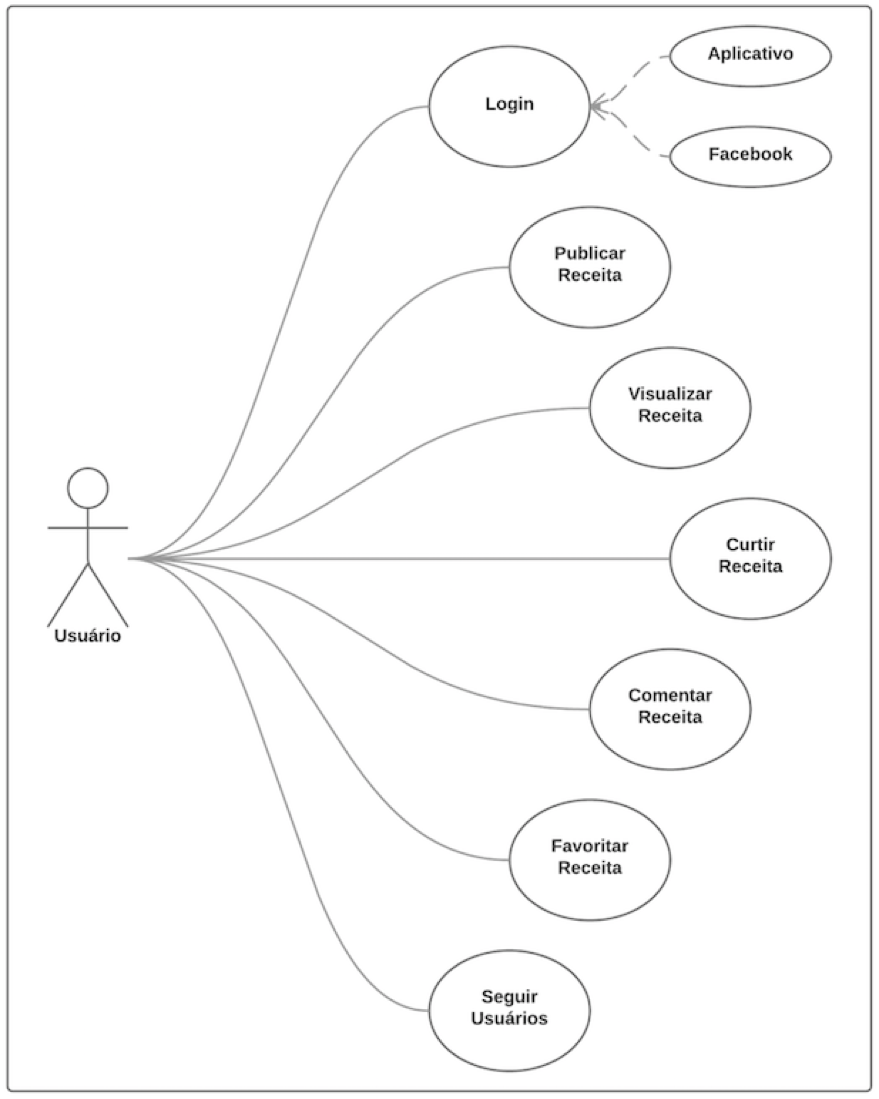
\includegraphics[scale=0.7]{imagens/figura8.png}
	\legend{Fonte: Elaborada pelo autor}
\end{figure}


\subsubsection{Descrição dos casos de uso} \label{sec:vegood: descricao-dos casos-de-uso}

A partir do diagrama mostrado na Figura \ref{fig:diagrama-de-caso-de-uso}, foram criados os seguintes casos de uso:

\begin{lista}
	\item \textbf{Caso de Uso 01 - LOGIN};
	\item \textbf{Caso de Uso 02 - PUBLICAR RECEITA};
	\item \textbf{Caso de Uso 03 - VISUALIZAR RECEITA};
	\item \textbf{Caso de Uso 04 - CURTIR RECEITA};
	\item \textbf{Caso de Uso 05 - COMENTAR RECEITA};
	\item \textbf{Caso de Uso 06 - FAVORITAR RECEITA};
	\item \textbf{Caso de Uso 07 - SEGUIR USUÁRIOS};
\end{lista}

Os documentos com as especificações completas estão disponíveis no apêndice \ref{apendice:a} deste trabalho.


\subsection{Diagrama de Classes}

O Diagrama de Classes descreve, em seu conteúdo, as classes e os seus relacionamentos. Em adendo, apresenta ainda o modelo de dados físico do aplicação, Figura \ref{fig:diagrama-de-classes}.

\begin{figure}[H]
	\caption{\label{fig:diagrama-de-classes}Diagrama de classes do Vegood}
	\centering
	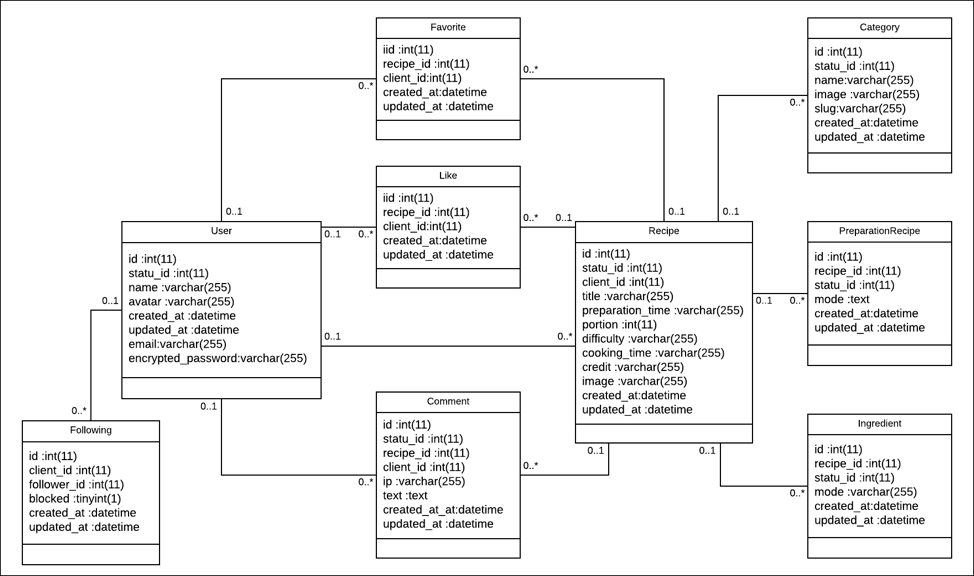
\includegraphics[scale=0.9]{imagens/figura9.png}
	\legend{Fonte: Elaborada pelo autor}
\end{figure}



\section{Desenvolvimento}
Nesta seção apresentamos uma visão dos passos e estrutura de projeto utilizando o framework híbrido Ionic. 


\subsection{Preparando o ambiente de trabalho} \label{sec:vegood:Funcionalidades}
Na implementação do código fonte foi utilizado o Sublime Text 3, um editor de texto projetado para ser simples, rápido, flexível e fácil de usar. Registramos que foram requeridas algumas dependências no desenvolvimento deste projeto. 

A seguir, serão descritas, de forma sequencial, as etapas necessárias a preparação do ambiente de trabalho.

Para obter o Ionic, precisamos do Node.JS, que é uma plataforma de desenvolvimento de aplicações utilizando Javascript, instalado na máquina, pois o processo é feito via NPM, um gerador de pacotes do Node.Js . Após instalar o Node.JS com sucesso, é indicado que se adicione os SDKs (\textit{Software Development Kit}) da(s) plataforma(s) com que se deseja trabalhar (Android, IOS, Windows Phone). Cada plataforma possui um processo de instalação diferenciado, lembrando que para utilizar e compilar versões para iOS é necessário que se utilize um notebook da linha Mac, do fabricante Apple. Com o Node.Js instalado, o utilitário terminal deve ser utilizado para a instalação do Ionic, através do comando ”npm install  -g ionic”. Ao final desta execução o ambiente Ionic torna-se disponível e acessível por meio do comando externo “ionic”. Para uma confirmação, a execução do comando “ionic --version“, exibe a versão instalada.

Usando o gerador do Ionic CLI para a criação de um novo projeto, informamos o template desejado e um modelo é gerado com os componentes iniciais do template escolhido. Para tal é utilizado o seguinte comando: “ionic start nomedoapp [template]“, onde tabs é o parâmetro padrão para template , que pode ser substituído pelos parâmetros sidemenu ou blank.

Para testar o aplicativo, o Ionic  CLI disponibiliza o comando “ionic serve [opção]“ que inicia um servidor de desenvolvimento local que pode ser visualizado em seu navegador padrão.. Esse comando também inicia o Live Reload, recurso que é utilizado para monitorar as mudanças feitas na aplicação. Com ele, qualquer alteração no arquivo do projeto irá atualizar automaticamente o browser. Uma opção adicional para a  visualização do projeto é o comando “ionic serve --lab“, que simula as telas em Android e IOS, lado a lado.

Após as etapas descritas acima, o ambiente se encontra pronto para o inicio do desenvolvimento.

\subsubsection{Estrutura do sistema}
Em um projeto utilizando Ionic Framework é gerada uma estrutura de diretórios, comum a todos os projetos (Figura 10).

\begin{figure}[H]
	\caption{\label{fig:estrutura-de-diretorios-do-projeto}Estrutura de diretórios do projeto Vegood}
	\centering
	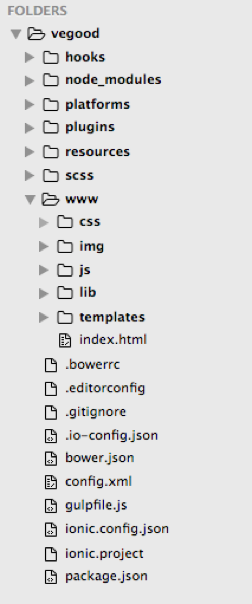
\includegraphics[scale=1]{imagens/figura10.png}
	\legend{Fonte: Elaborado pelo autor}
\end{figure}


\subsection{Interface do aplicativo}
Descrevemos as principais telas da interface gráfica da aplicação Vegood.

\subsubsection{Tela de login}
Logo que a aplicação é aberta, a tela de login é apresentada e o usuário tem 3 possibilidades de ação: 
\begin{lista}
	\item Fazer o login pelo próprio aplicativo (usando os dados necessários, se já possuir uma conta);
	\item fazer login usando o facebook (onde o aplicativo pede autorização para usar as credenciais do facebook para prosseguir o acesso ao aplicativo);
	\item  Criar uma nova conta;
\end{lista}

\begin{figure}[H]
	\caption{\label{fig:tela-de-login}Tela de login}
	\centering
	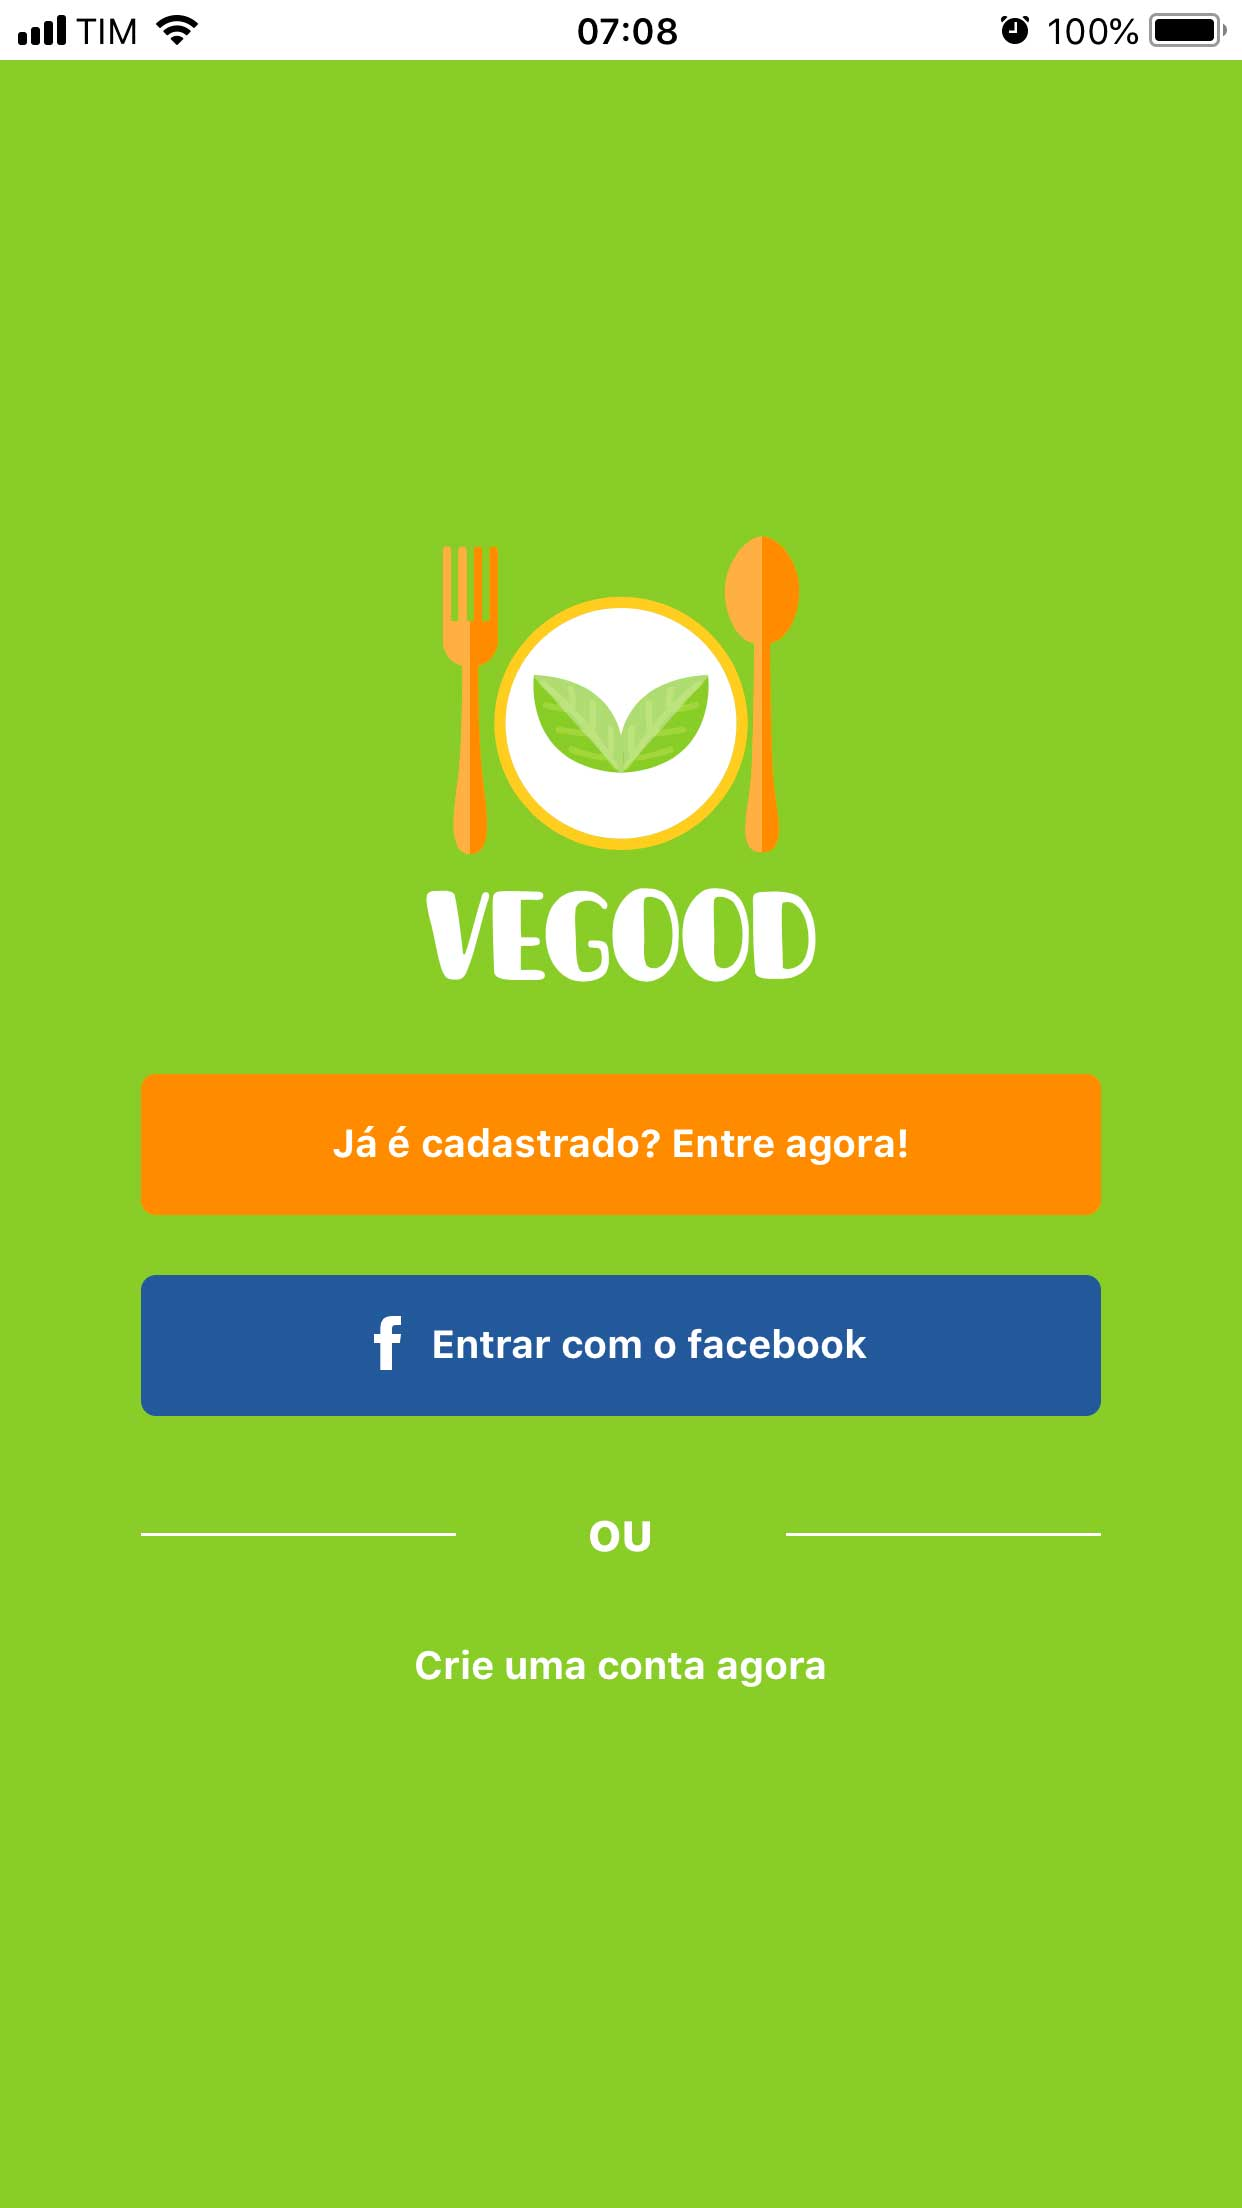
\includegraphics[scale=0.15]{imagens/figura11.jpg}
\end{figure}




\subsubsection{Tela de cadastro}
Essa tela por meio da qual o usuário cria sua conta para ter acesso e usufruir de todas funcionalidades do aplicativo. Com exceção de cadastrar a foto de perfil, todos os campos são obrigatórios e devem ser preenchidos para a conclusão do cadastro.

\begin{figure}[H]
	\caption{\label{fig:tela-de-1}Tela de cadastro}
	\centering
	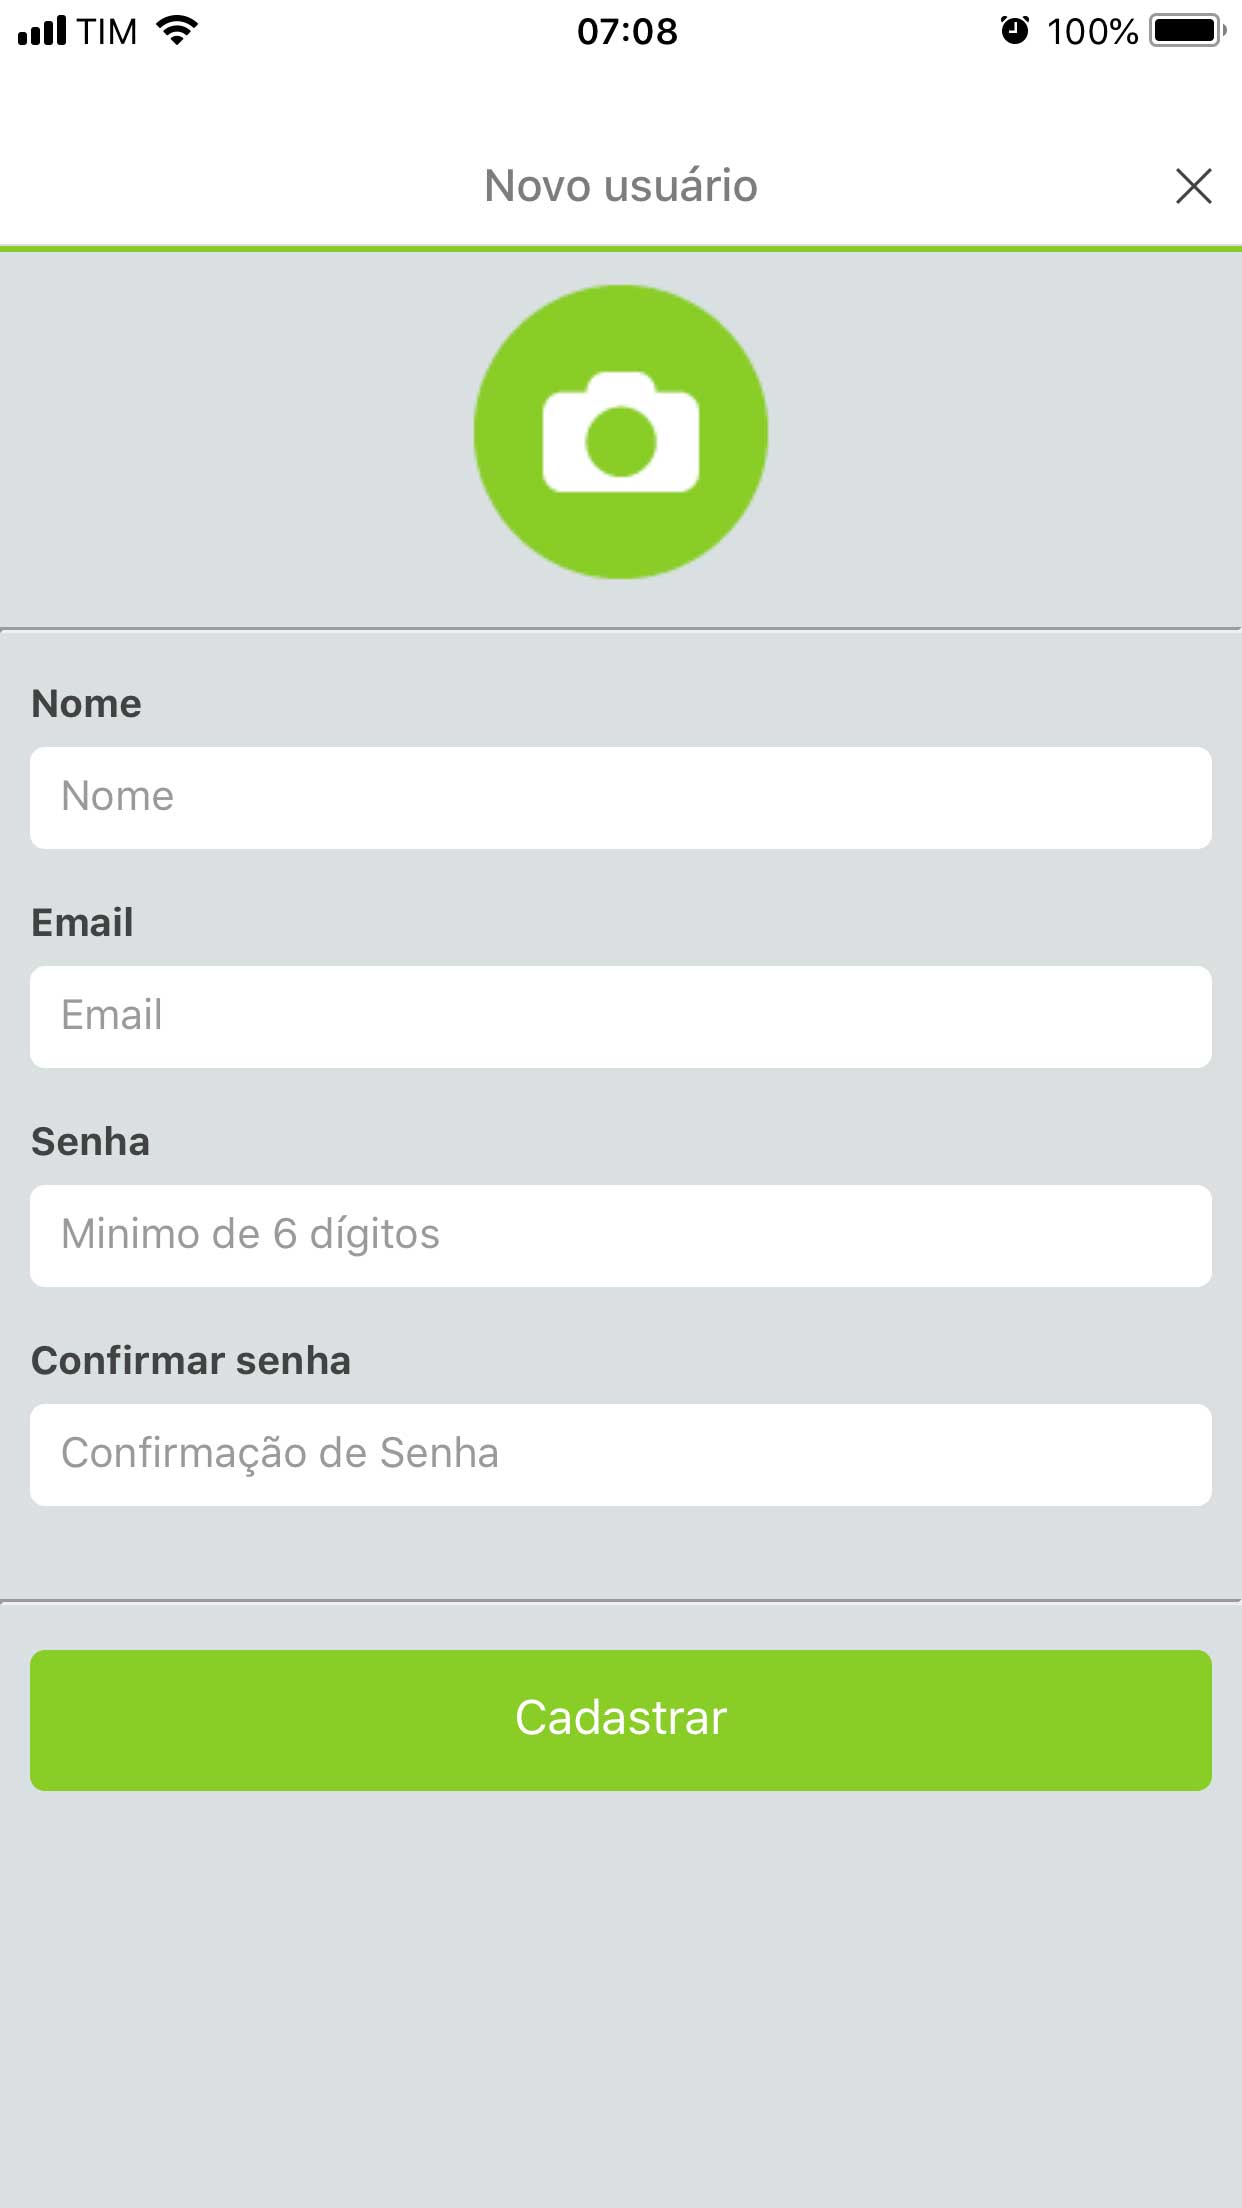
\includegraphics[scale=0.15]{imagens/figura12.jpg}
\end{figure}



\subsubsection{Tela principal}
Após a autenticação do usuário, a aplicação apresenta a tela principal com um \textit{feed} de receitas publicadas, onde o usuário pode interagir com as mesmas, clicando no nome do usuário que publicou a receita e se encaminhando ao seu perfil. Com apenas  um clique, o usuário também pode curtir, comentar e até mesmo favoritar as receitas. Além disso, para obter mais informações de uma determinada receita, basta clicar em uma delas e uma nova tela surge, com todas as informações.

Nessa mesma tela, também podemos ver um menu em tabs na parte inferior do aplicativo, que representam as opções de exibições: Inicio, Categorias, Enviar receita, Conta e Mais.

\begin{figure}[H]
	\caption{\label{fig:tela-de-2}Tela principal}
	\centering
	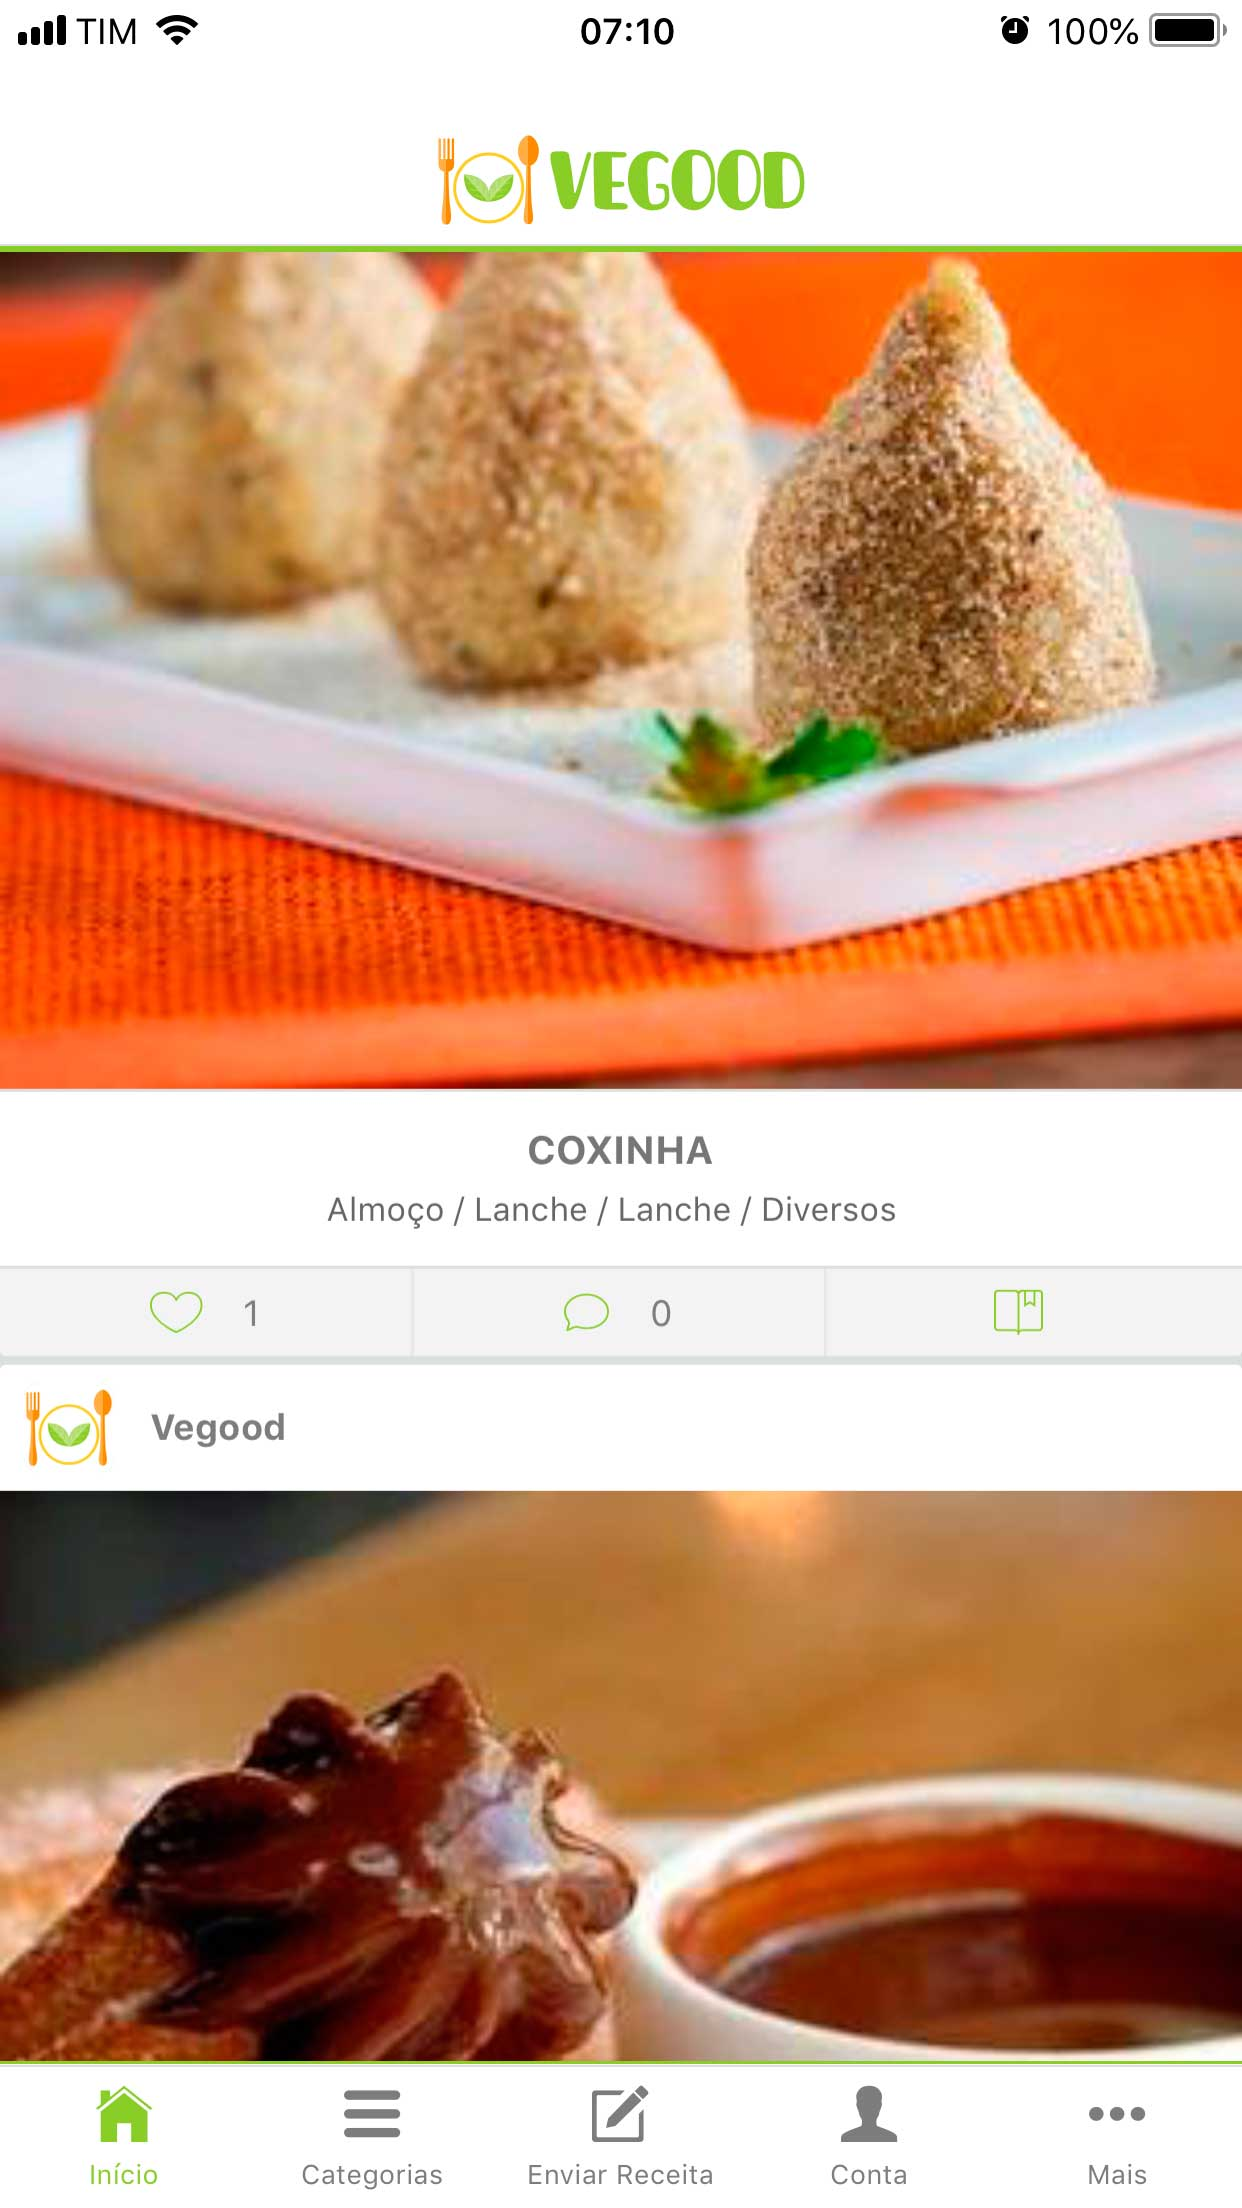
\includegraphics[scale=0.15]{imagens/figura13.jpg}
\end{figure}

\subsubsection{Tela interna de uma receita}
Nessa tela, o usuário pode fazer praticamente as mesmas coisas da tela principal, podendo clicar no nome do usuário que publicou a receita e ir para o seu perfil. Com um clique, o usuário também pode curtir, comentar e até mesmo favoritar as receitas. A parte mais importante dessa tela são as informações sobre a receita, onde o usuário pode ver, por exemplo, o tempo de preparo e cozimento, o rendimento e a dificuldade, além de ter todas as informações de ingredientes necessários e modo de preparo para fazer a receita.

\begin{figure}[H]
	\caption{\label{fig:tela-de-3}Tela interna de uma receita}
	\centering
	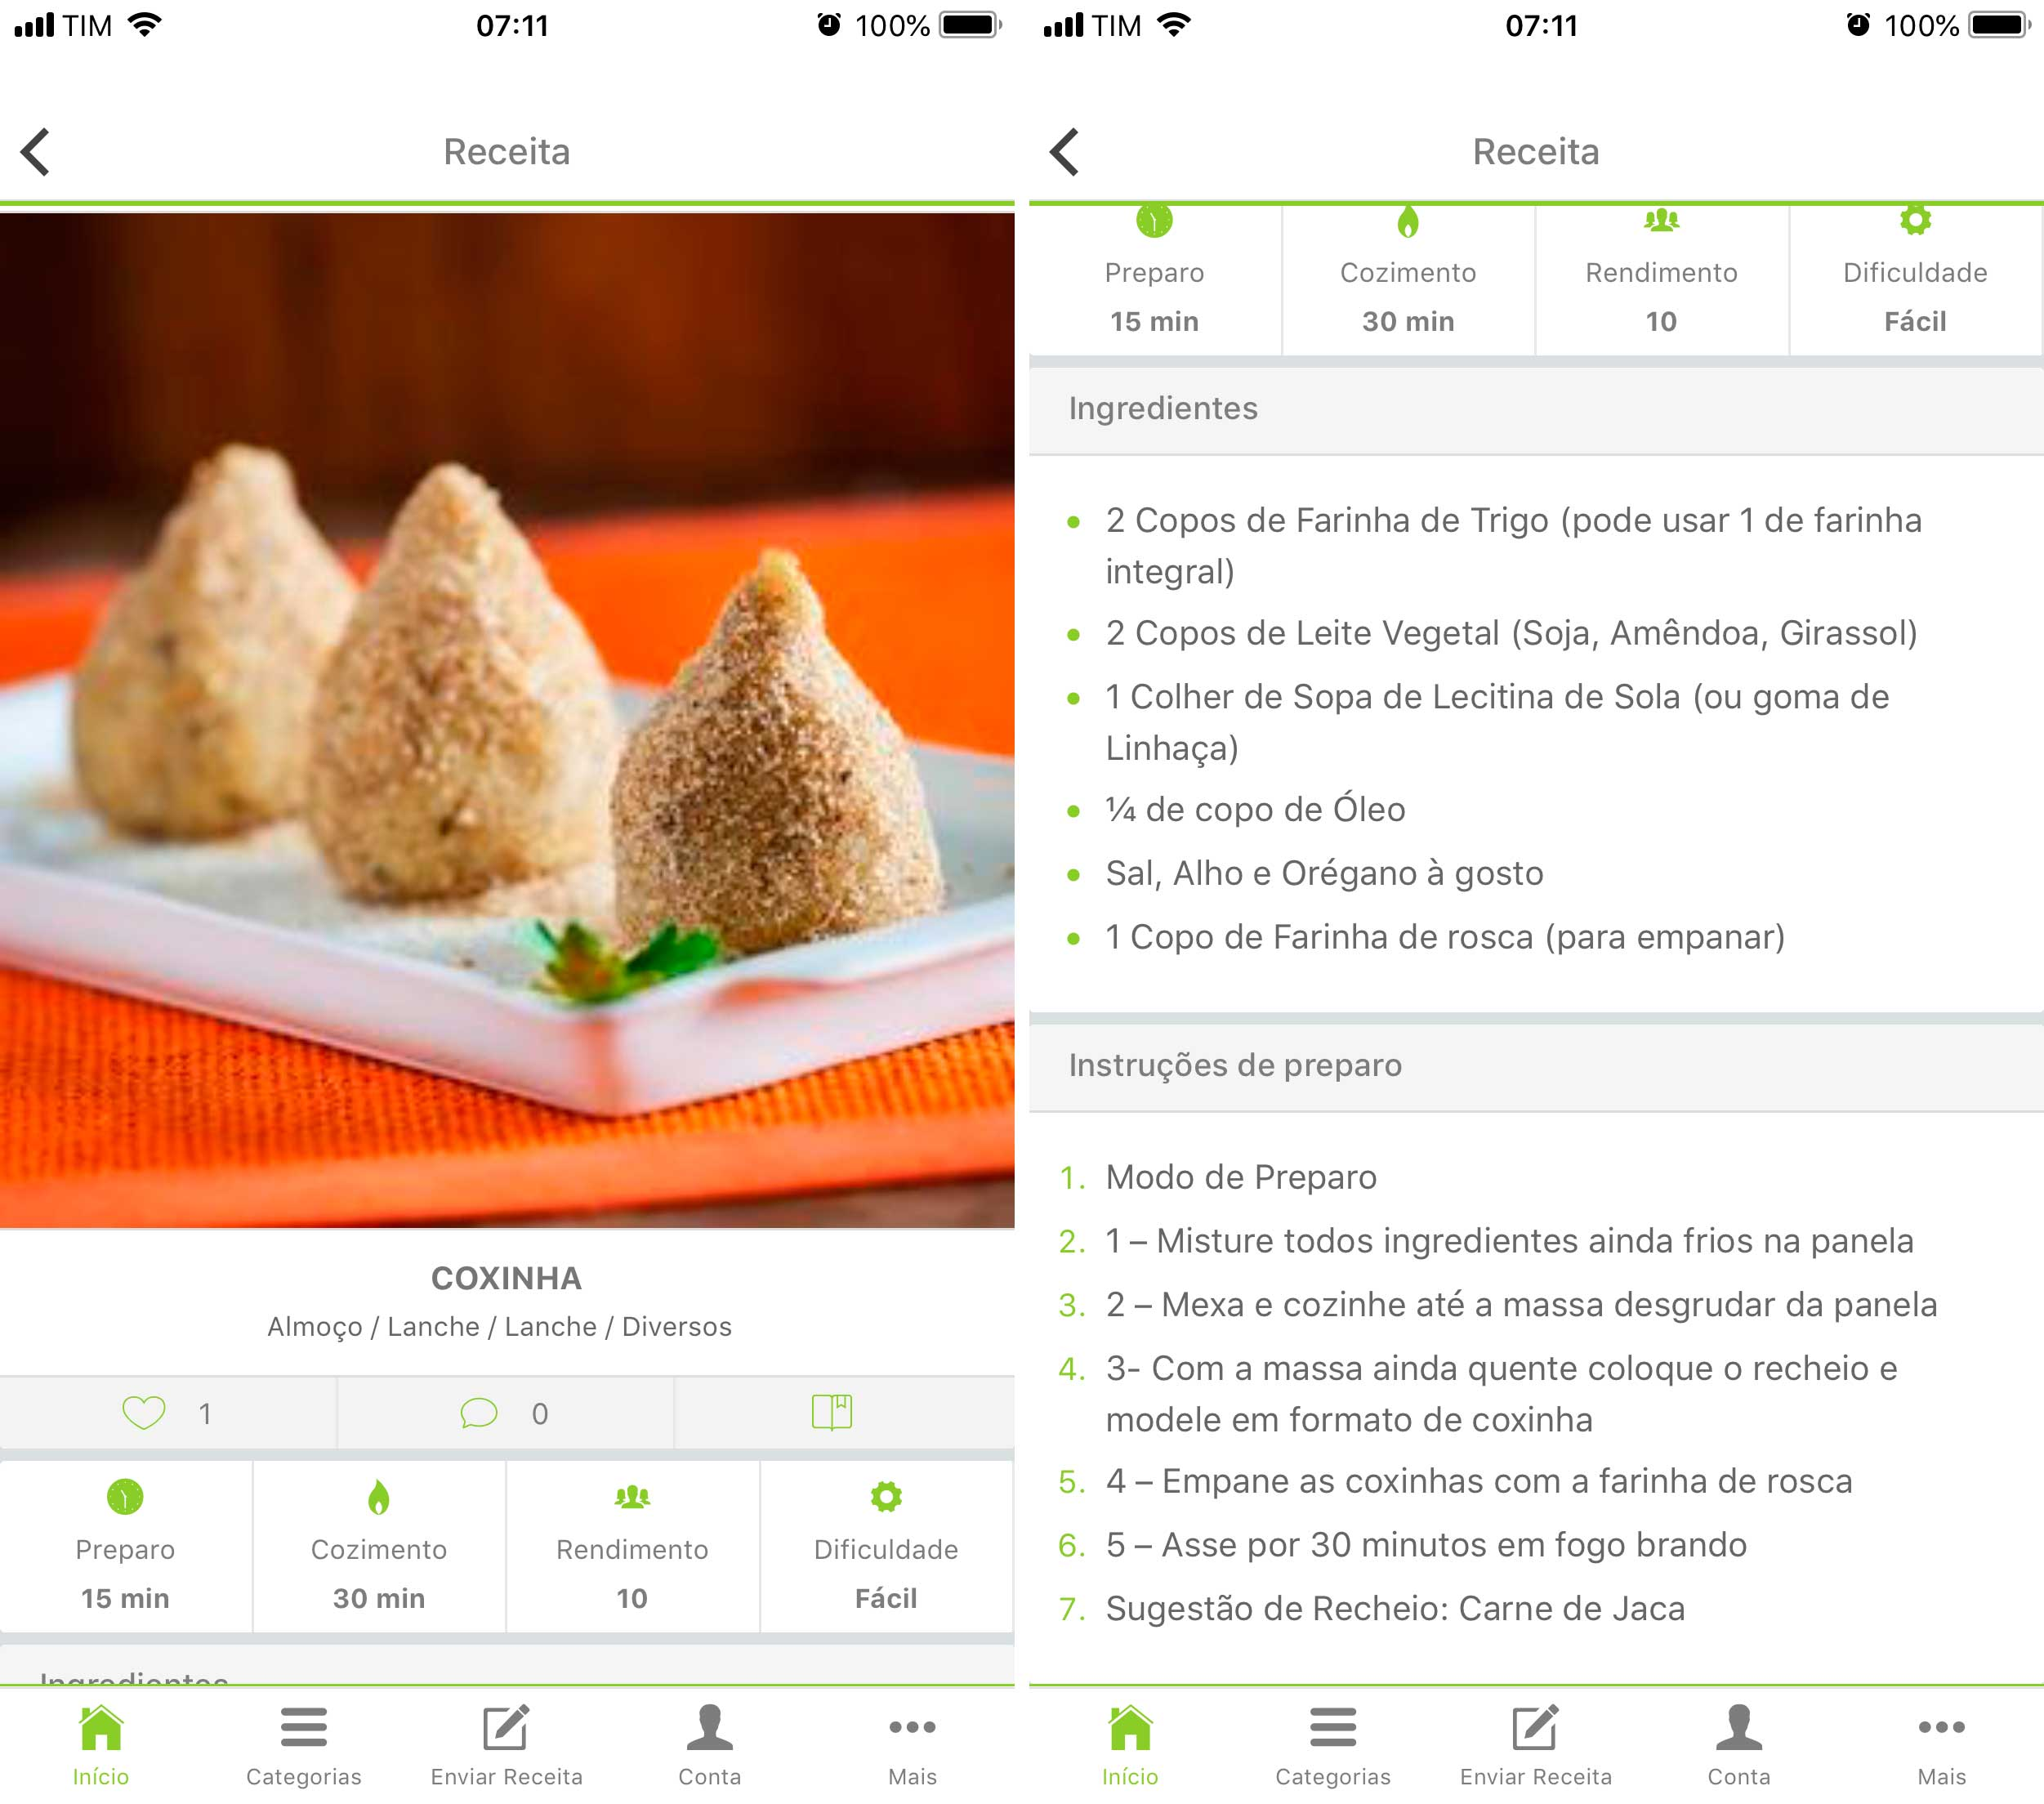
\includegraphics[scale=0.15]{imagens/figura14.jpg}
\end{figure}

\subsubsection{Tela de categorias}
Na tela de categorias o usuário tem disponível 5 categorias: almoço, café da manhã, jantar, lanche e outros. Com as categorias divididas dessa forma, fica facilitada a localização de alguma receita, de acordo com o tipo de refeição que se deseja  aprender.

Ao se clicar em uma categoria uma nova tela é apresentada, contendo todas as receitas relacionadas à categoria selecionada e, na parte superior, a quantidade de receitas que aquela categoria possui

\begin{figure}[H]
	\caption{\label{fig:tela-de-4}Tela de categorias}
	\centering
	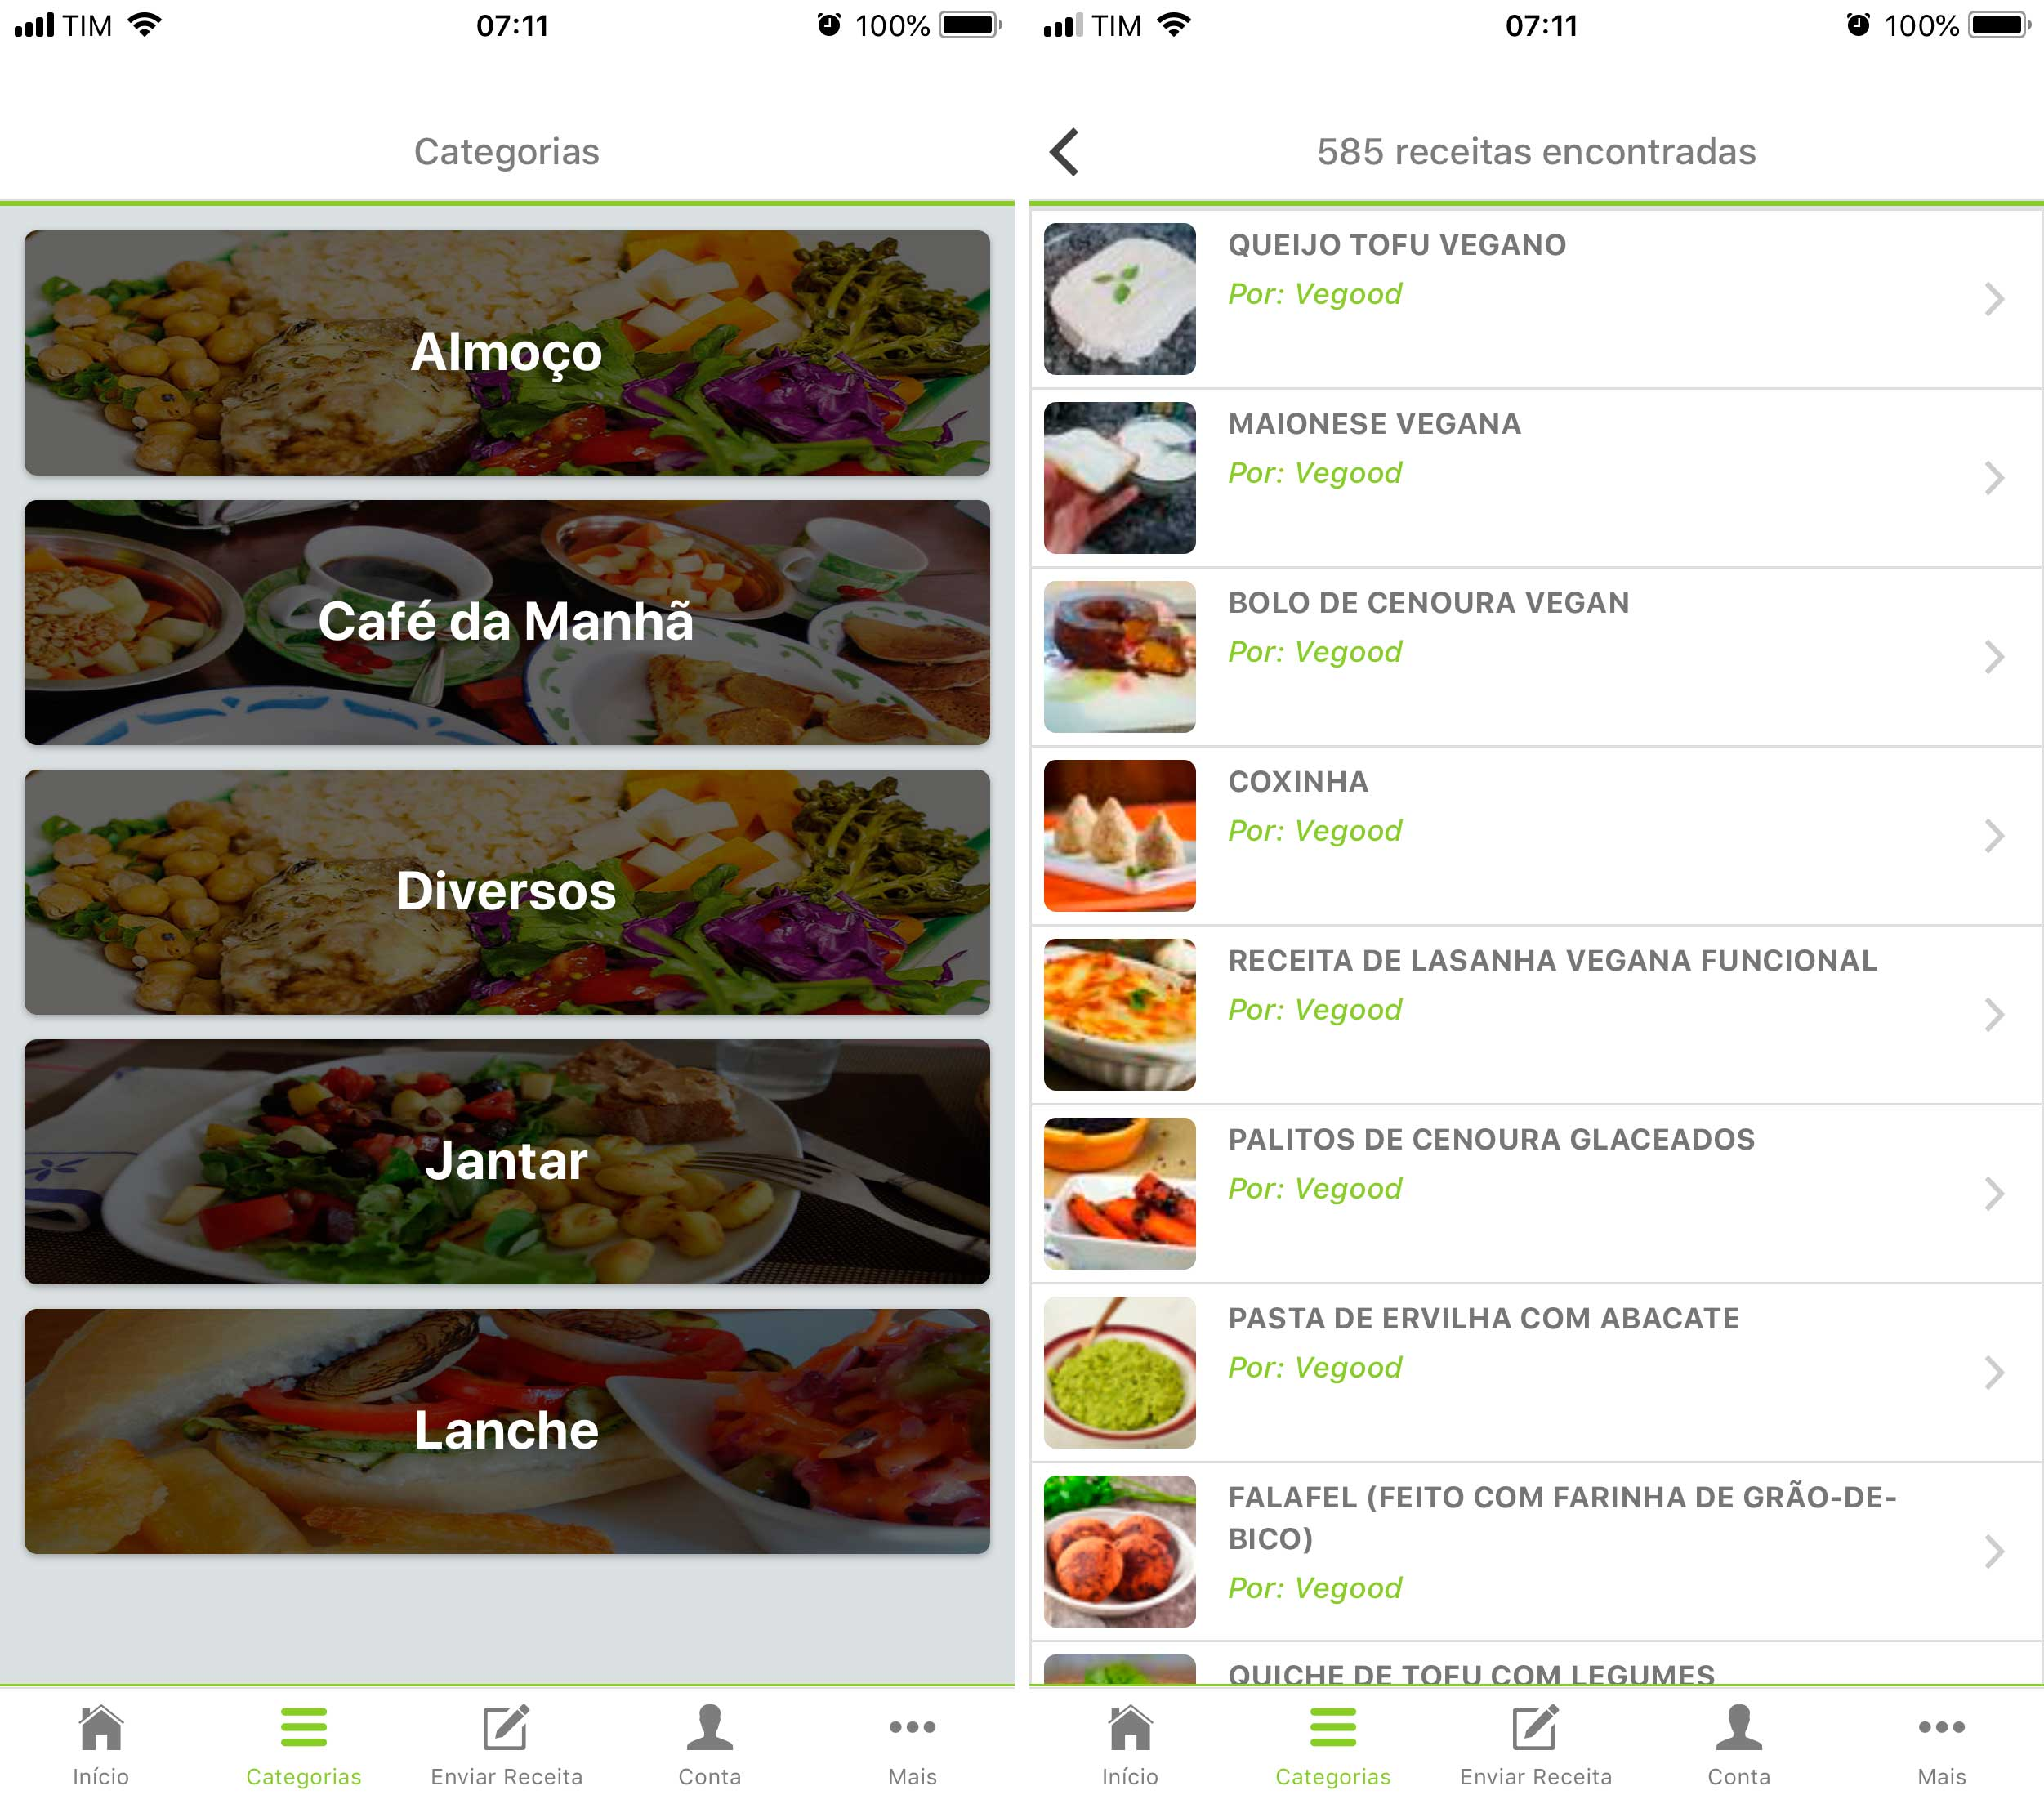
\includegraphics[scale=0.15]{imagens/figura15.jpg}
\end{figure}

\subsubsection{Tela de enviar uma receita}
Na tela de enviar receita, o usuário tem disponível um formulário bem simples e objetivo com os campos necessários para publicar uma receita. Nesse formulário  há a possibilidade de se usar a câmera do próprio celular para capturar uma foto ou selecionar dos seus arquivos uma imagem para a receita. O usuário, além da foto, pode cadastrar de forma prática e direta o nome da receita, como também selecionar uma ou mais categorias, tempo de preparo, tempo de cozimento, rendimento, dificuldade de execução, os ingredientes e o modo de preparo.

\begin{figure}[H]
	\caption{\label{fig:tela-de-5}Tela de enviar uma receita}
	\centering
	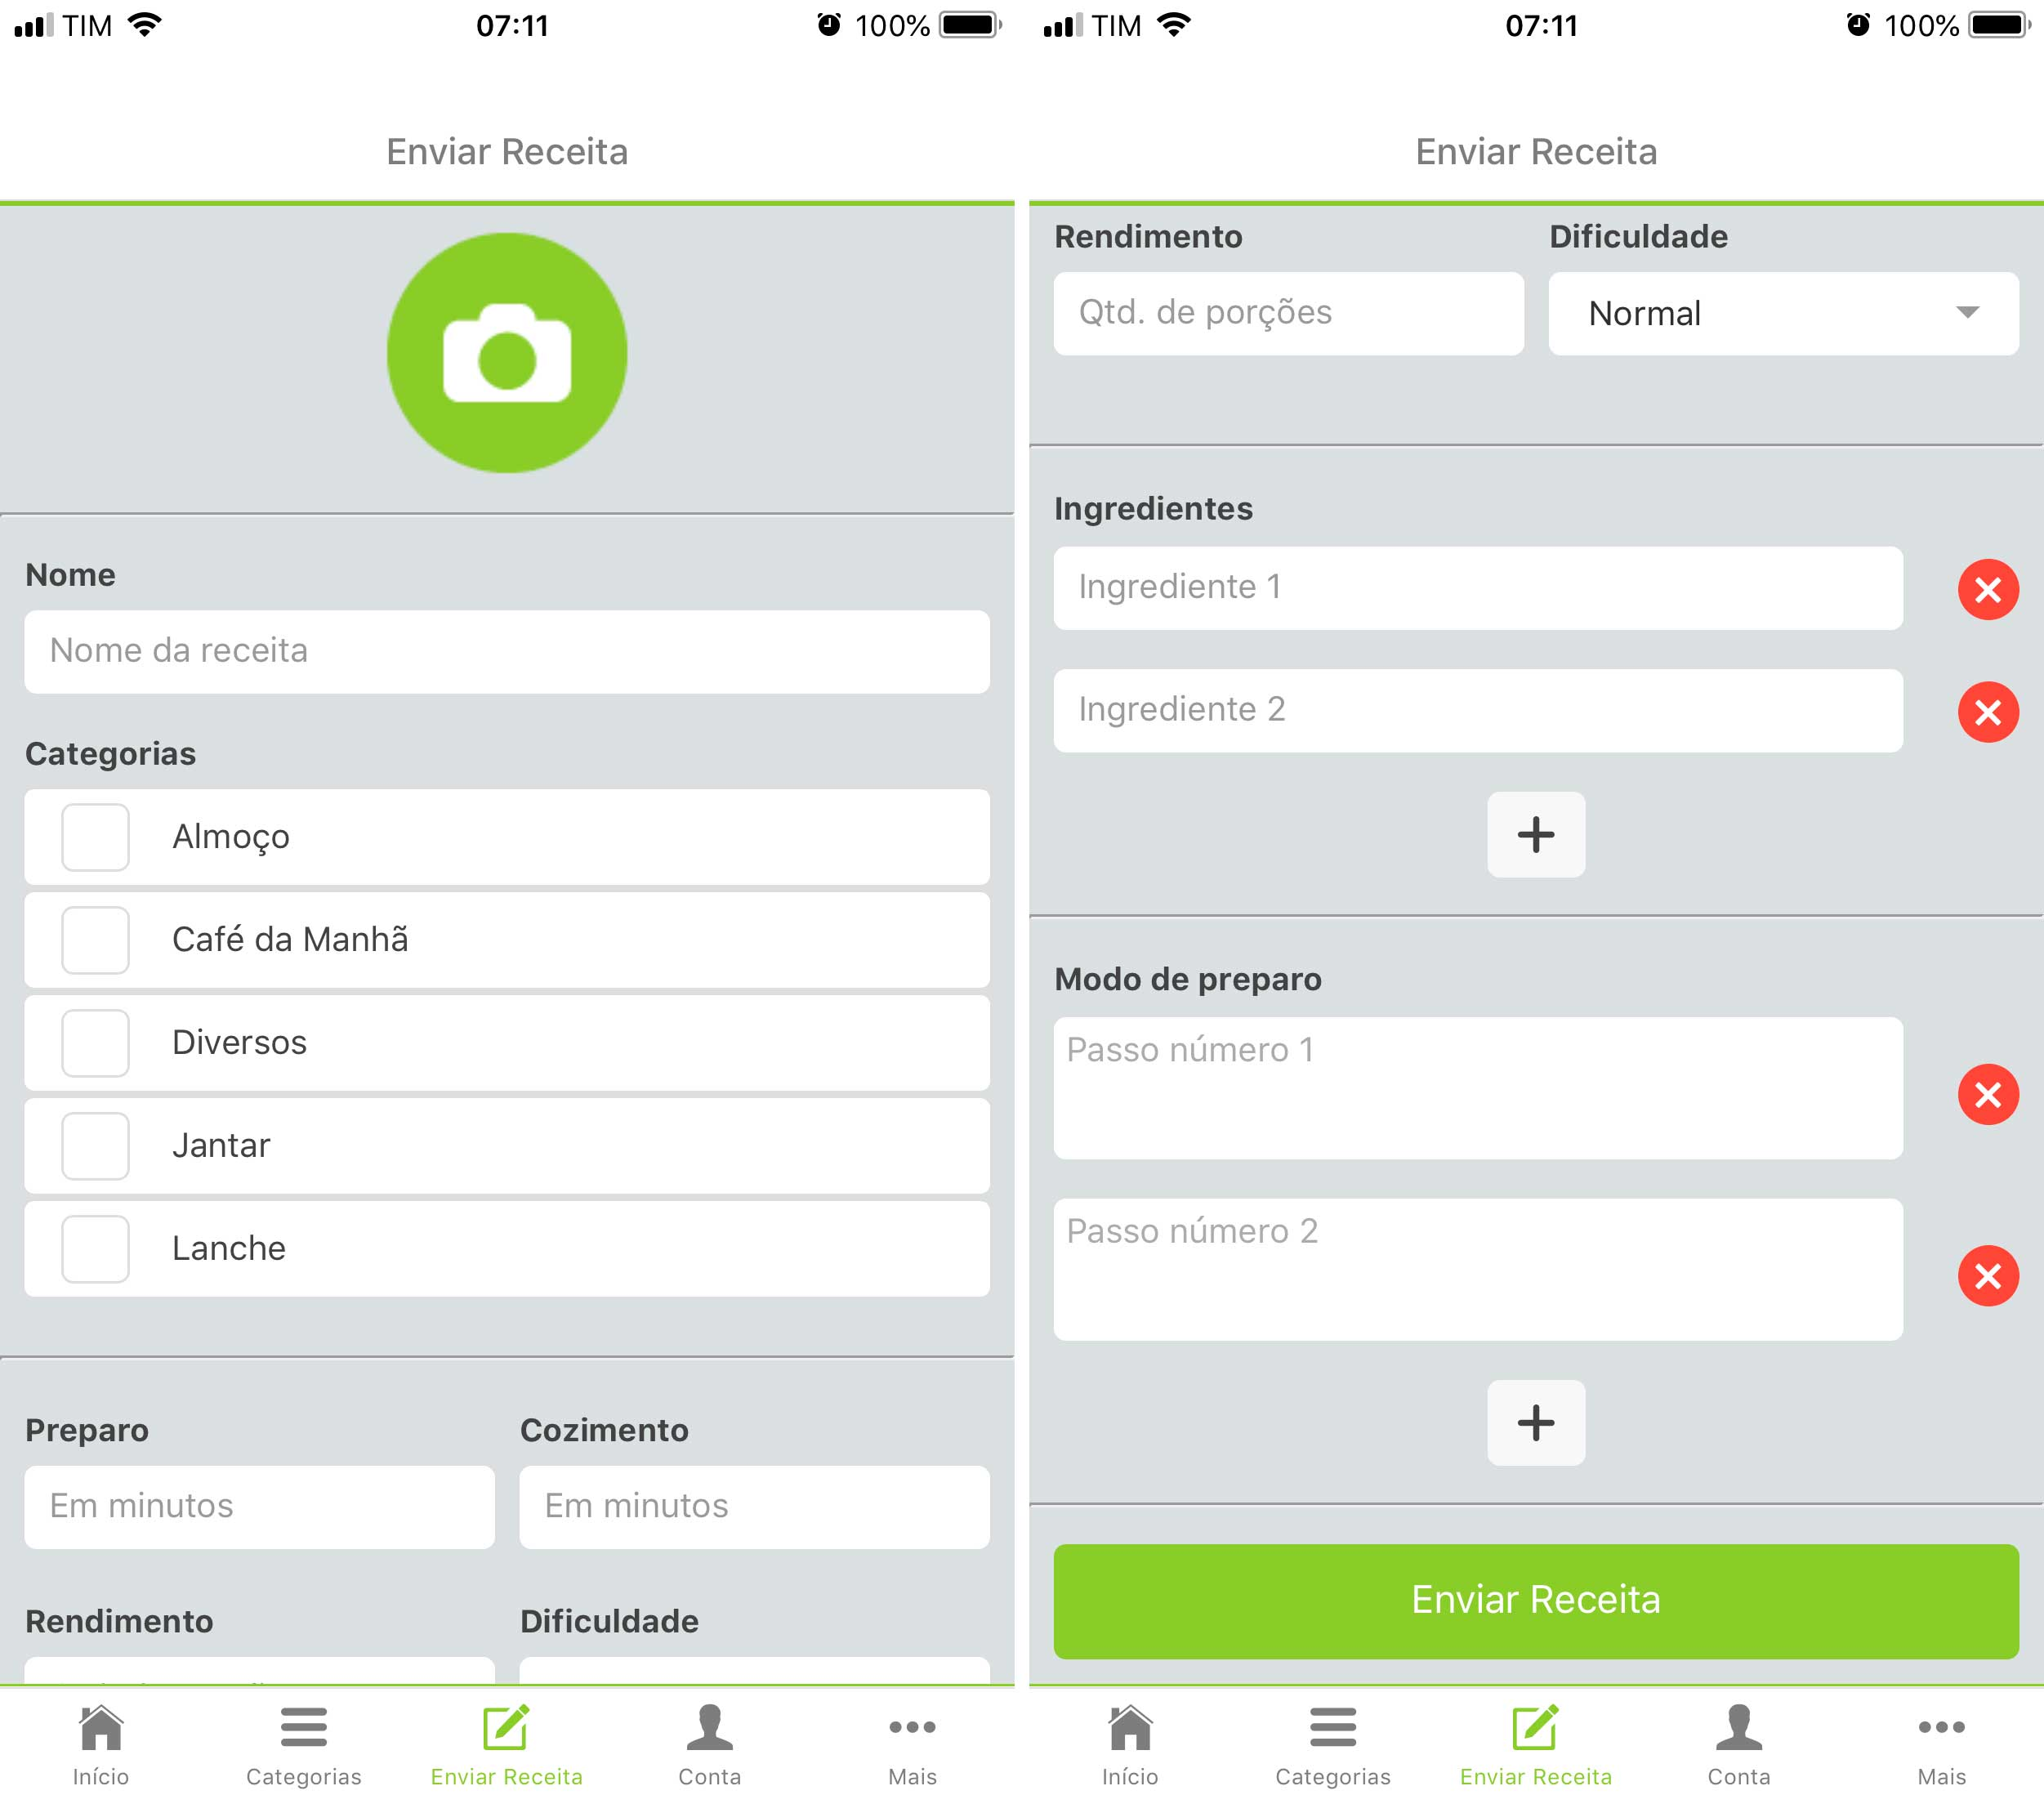
\includegraphics[scale=0.15]{imagens/figura16.jpg}
\end{figure}

\subsubsection{Tela de perfil}
A tela de perfil é bem simples. O usuário pode ver as receitas que favoritou bem como editar o seu próprio perfil. É possível ainda ver a quantidade a lista das receitas que publicou,os seus seguidores e a quem está seguindo.

No topo da tela existe uma opção para edição dos seus dados pessoais.

\begin{figure}[H]
	\caption{\label{fig:tela-de-6}Tela de perfil}
	\centering
	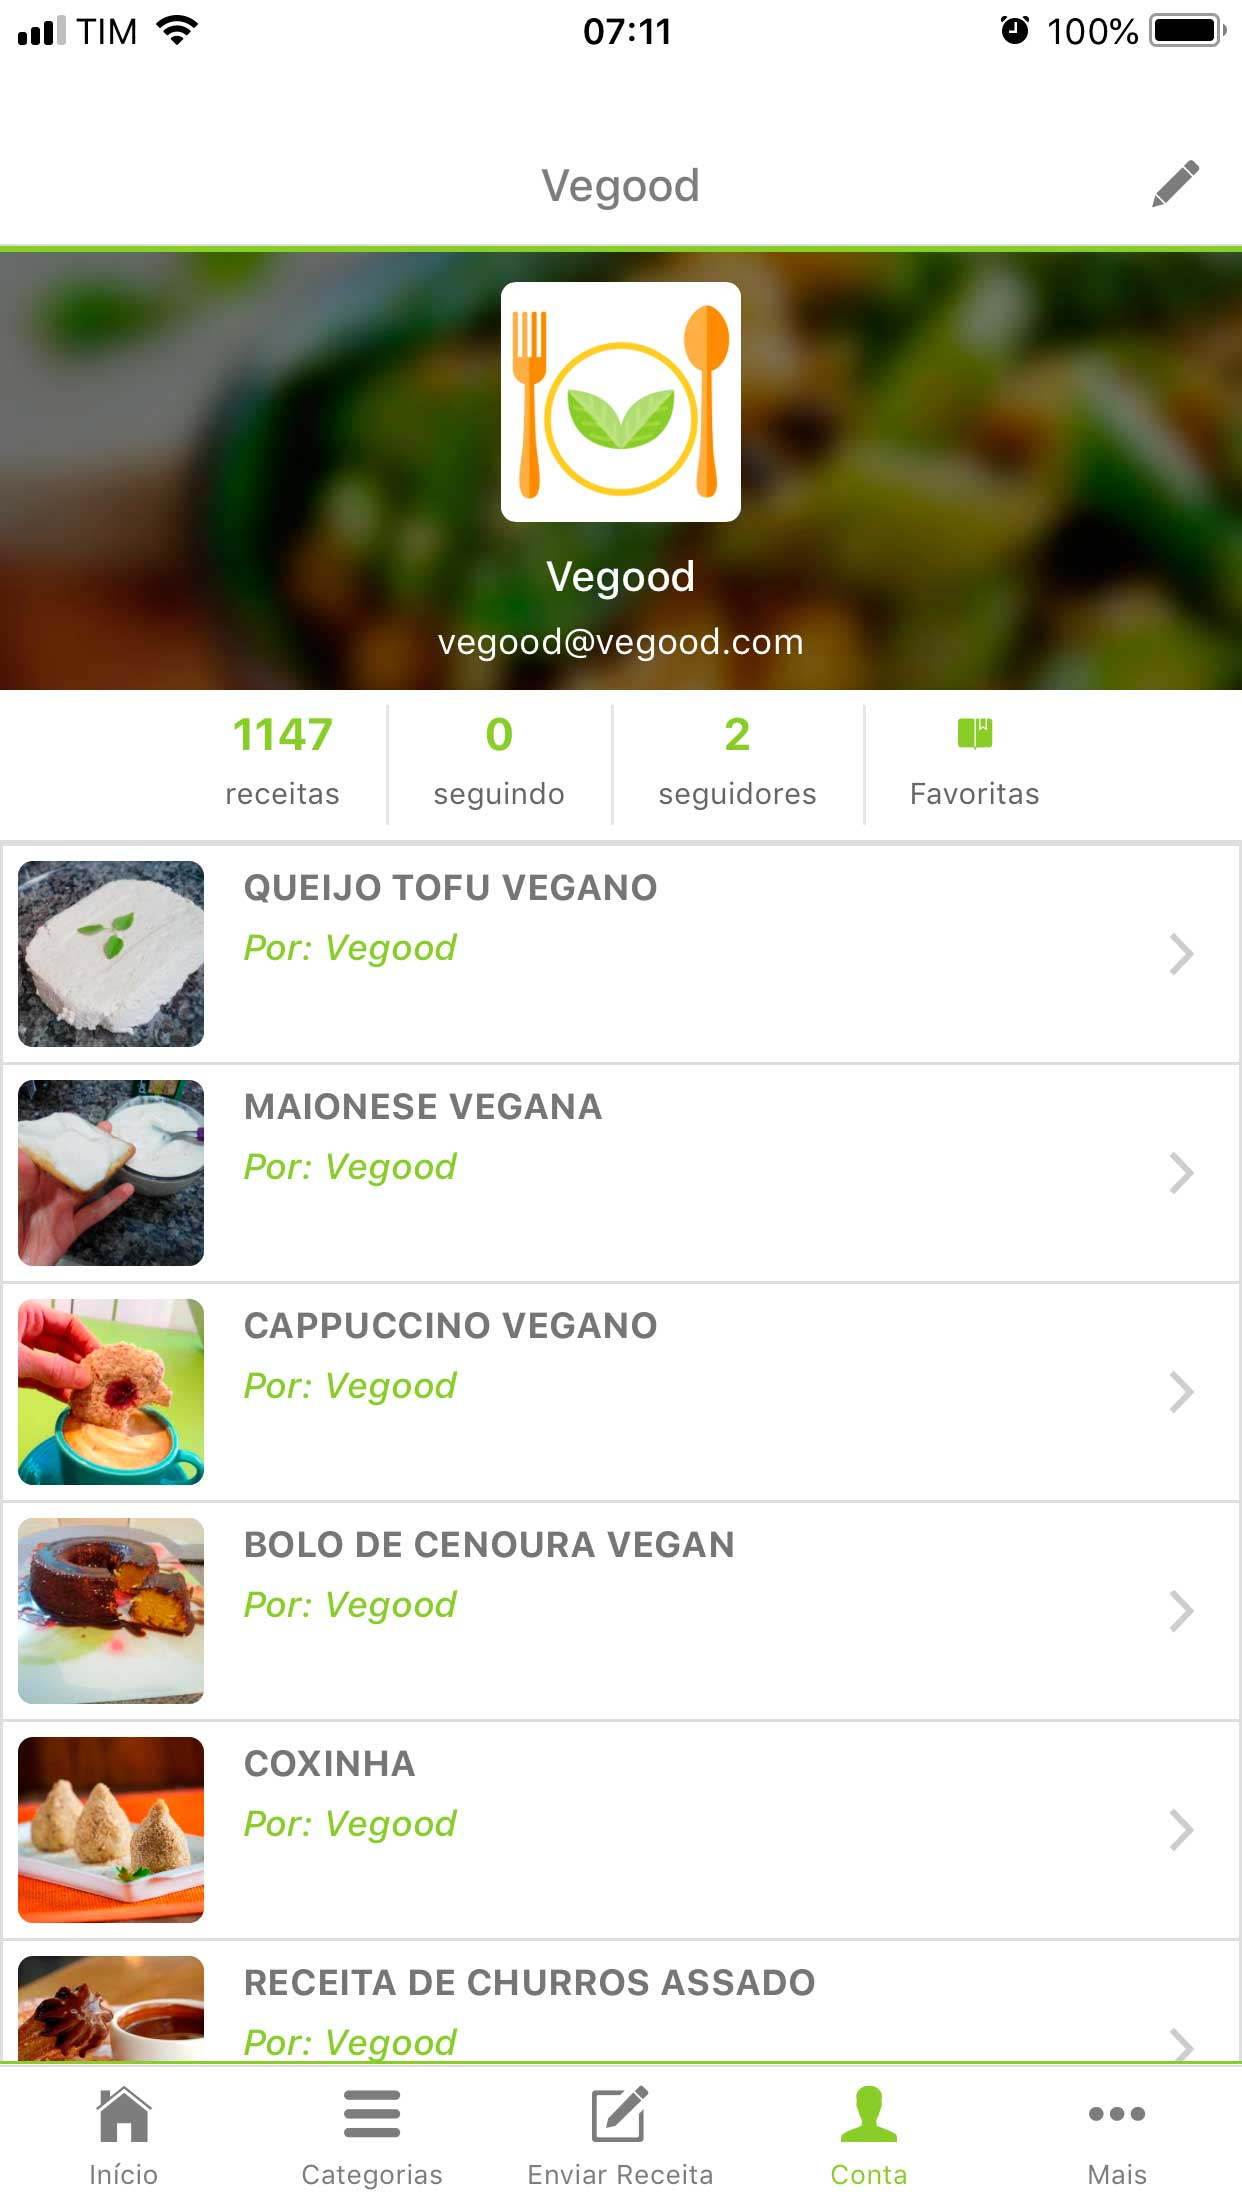
\includegraphics[scale=0.15]{imagens/figura17.jpg}
\end{figure}
